\begin{figure*}[t]
\centering
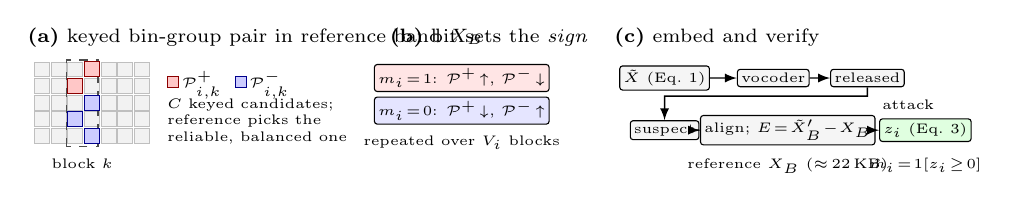
\begin{tikzpicture}[
  scale=0.92,
  x=1mm,y=1mm,
  font=\scriptsize,
  box/.style={draw,rounded corners=1pt,inner sep=1.4pt,align=center,font=\tiny},
  pgrp/.style={fill=red!22,draw=red!55!black,line width=.25pt},
  ngrp/.style={fill=blue!20,draw=blue!55!black,line width=.25pt},
  cell/.style={draw=black!25,line width=.15pt,fill=black!5},
  ar/.style={-latex,line width=.5pt},
]
% ---------- (a) reference band with bin-group pair ----------
\node[anchor=south west,inner sep=0] at (-1,13.2)
  {\textbf{(a)} keyed bin-group pair in reference band $X_B$};
\foreach \c in {0,...,6}{\foreach \r in {0,...,4}{
  \fill[cell] (\c*2.3,\r*2.3) rectangle ++(2.05,2.05);}}
\draw[black!70,line width=.5pt,dashed] (4.4,-.45) rectangle (8.8,11.5);
\node[anchor=north,font=\tiny] at (6.6,-.8) {block $k$};
\foreach \r in {3,1}{\fill[pgrp] (4.6,\r*2.3) rectangle ++(2.05,2.05);}
\fill[pgrp] (6.9,9.2) rectangle ++(2.05,2.05);
\foreach \r in {0,2}{\fill[ngrp] (6.9,\r*2.3) rectangle ++(2.05,2.05);}
\fill[ngrp] (4.6,2.3) rectangle ++(2.05,2.05);
\node[anchor=west,align=left,font=\tiny] at (17,8)
  {\tikz\fill[fill=red!22,draw=red!55!black,line width=.25pt](0,0)rectangle(1.4mm,1.4mm);\,$\mathcal{P}^+_{i,k}$\ \
   \tikz\fill[fill=blue!20,draw=blue!55!black,line width=.25pt](0,0)rectangle(1.4mm,1.4mm);\,$\mathcal{P}^-_{i,k}$};
\node[anchor=west,align=left,font=\tiny,text width=24mm] at (17,3)
  {$C$ keyed candidates;\\reference picks the\\reliable, balanced one};

% ---------- (b) sign encoding ----------
\node[anchor=south west,inner sep=0] at (49,13.2)
  {\textbf{(b)} bit sets the \emph{sign}};
\node[box,fill=red!10] at (59,9) {$m_i\!=\!1$: $\mathcal{P}^+\!\uparrow$, $\mathcal{P}^-\!\downarrow$};
\node[box,fill=blue!10] at (59,4.5) {$m_i\!=\!0$: $\mathcal{P}^+\!\downarrow$, $\mathcal{P}^-\!\uparrow$};
\node[anchor=north,align=center,font=\tiny] at (59,2.4) {repeated over $V_i$ blocks};

% ---------- (c) pipeline ----------
\node[anchor=south west,inner sep=0] at (80,13.2) {\textbf{(c)} embed and verify};
\node[box,fill=black!4] (mel)  at (87,9)    {$\tilde X$ (Eq.~1)};
\node[box,fill=black!4] (voc)  at (102,9)   {vocoder};
\node[box,fill=black!4] (wav)  at (115,9)   {released};
\node[box,fill=black!4] (susp) at (87,1.8)  {suspect};
\node[box,fill=black!4] (res)  at (104,1.8) {align; $E\!=\!\tilde X'_B\!-\!X_B$};
\node[box,fill=green!12] (z)   at (123,1.8) {$z_i$ (Eq.~3)};
\draw[ar] (mel) -- (voc);
\draw[ar] (voc) -- (wav);
\draw[ar] (susp) -- (res);
\draw[ar] (res) -- (z);
\draw[ar] (wav) -- ++(0,-2.5) -| (susp);
\node[anchor=west,font=\tiny] at (115.7,5.3) {attack};
\node[anchor=north,font=\tiny] at (104,-0.7) {reference $X_B$ ($\approx$\,22\,KB)};
\node[anchor=north,font=\tiny] at (123,-0.7) {$\hat m_i\!=\!\mathbb{1}[z_i\!\geq\!0]$};
\end{tikzpicture}
\caption{\texttt{RAWMER}. A bin-group pair is two disjoint groups of $P$ mel bins;
the bit is carried by the \emph{sign} of their energy difference, not by an absolute
pattern, so distortion common to both groups cancels in the score $z_i$.}
\label{fig:method}
\end{figure*}
